\chapter{Проблема проекции неба на плоскость}
\label{cha:ch_4}

Существует несколько способов преобразовать данные, записанные как координаты объектов в космических
координатах, в значения на плоскости, которые можно уложить на двумерную матрицу. При любой проекции 
сферы на плоскость мы будем сталкиваться с искажениями в разной степени и для разных параметров данных.

\section{HEALPix}
Этот формат является очень удобной формой хранения данных. Данные телескопа <<Планк>>, исследование
которых упоминается в обзоре существующих решений, хранятся именно в этом формате, поэтому над ними 
легко работать и для них не требуется такое количество стадий предобработки, как например для данных 
PS1. \\

Как ранее было упомянуто, HEALPix является иерархической структурой для хранения данных. Она 
позволяет сохранить на проекции площадь объекта, однако его форма может быть искажена. Таким образом,
задавая маски скоплений как круги, мы в большинстве случаев будем наблюдать их искажение до эллипсов.\\

\begin{figure}
    \center{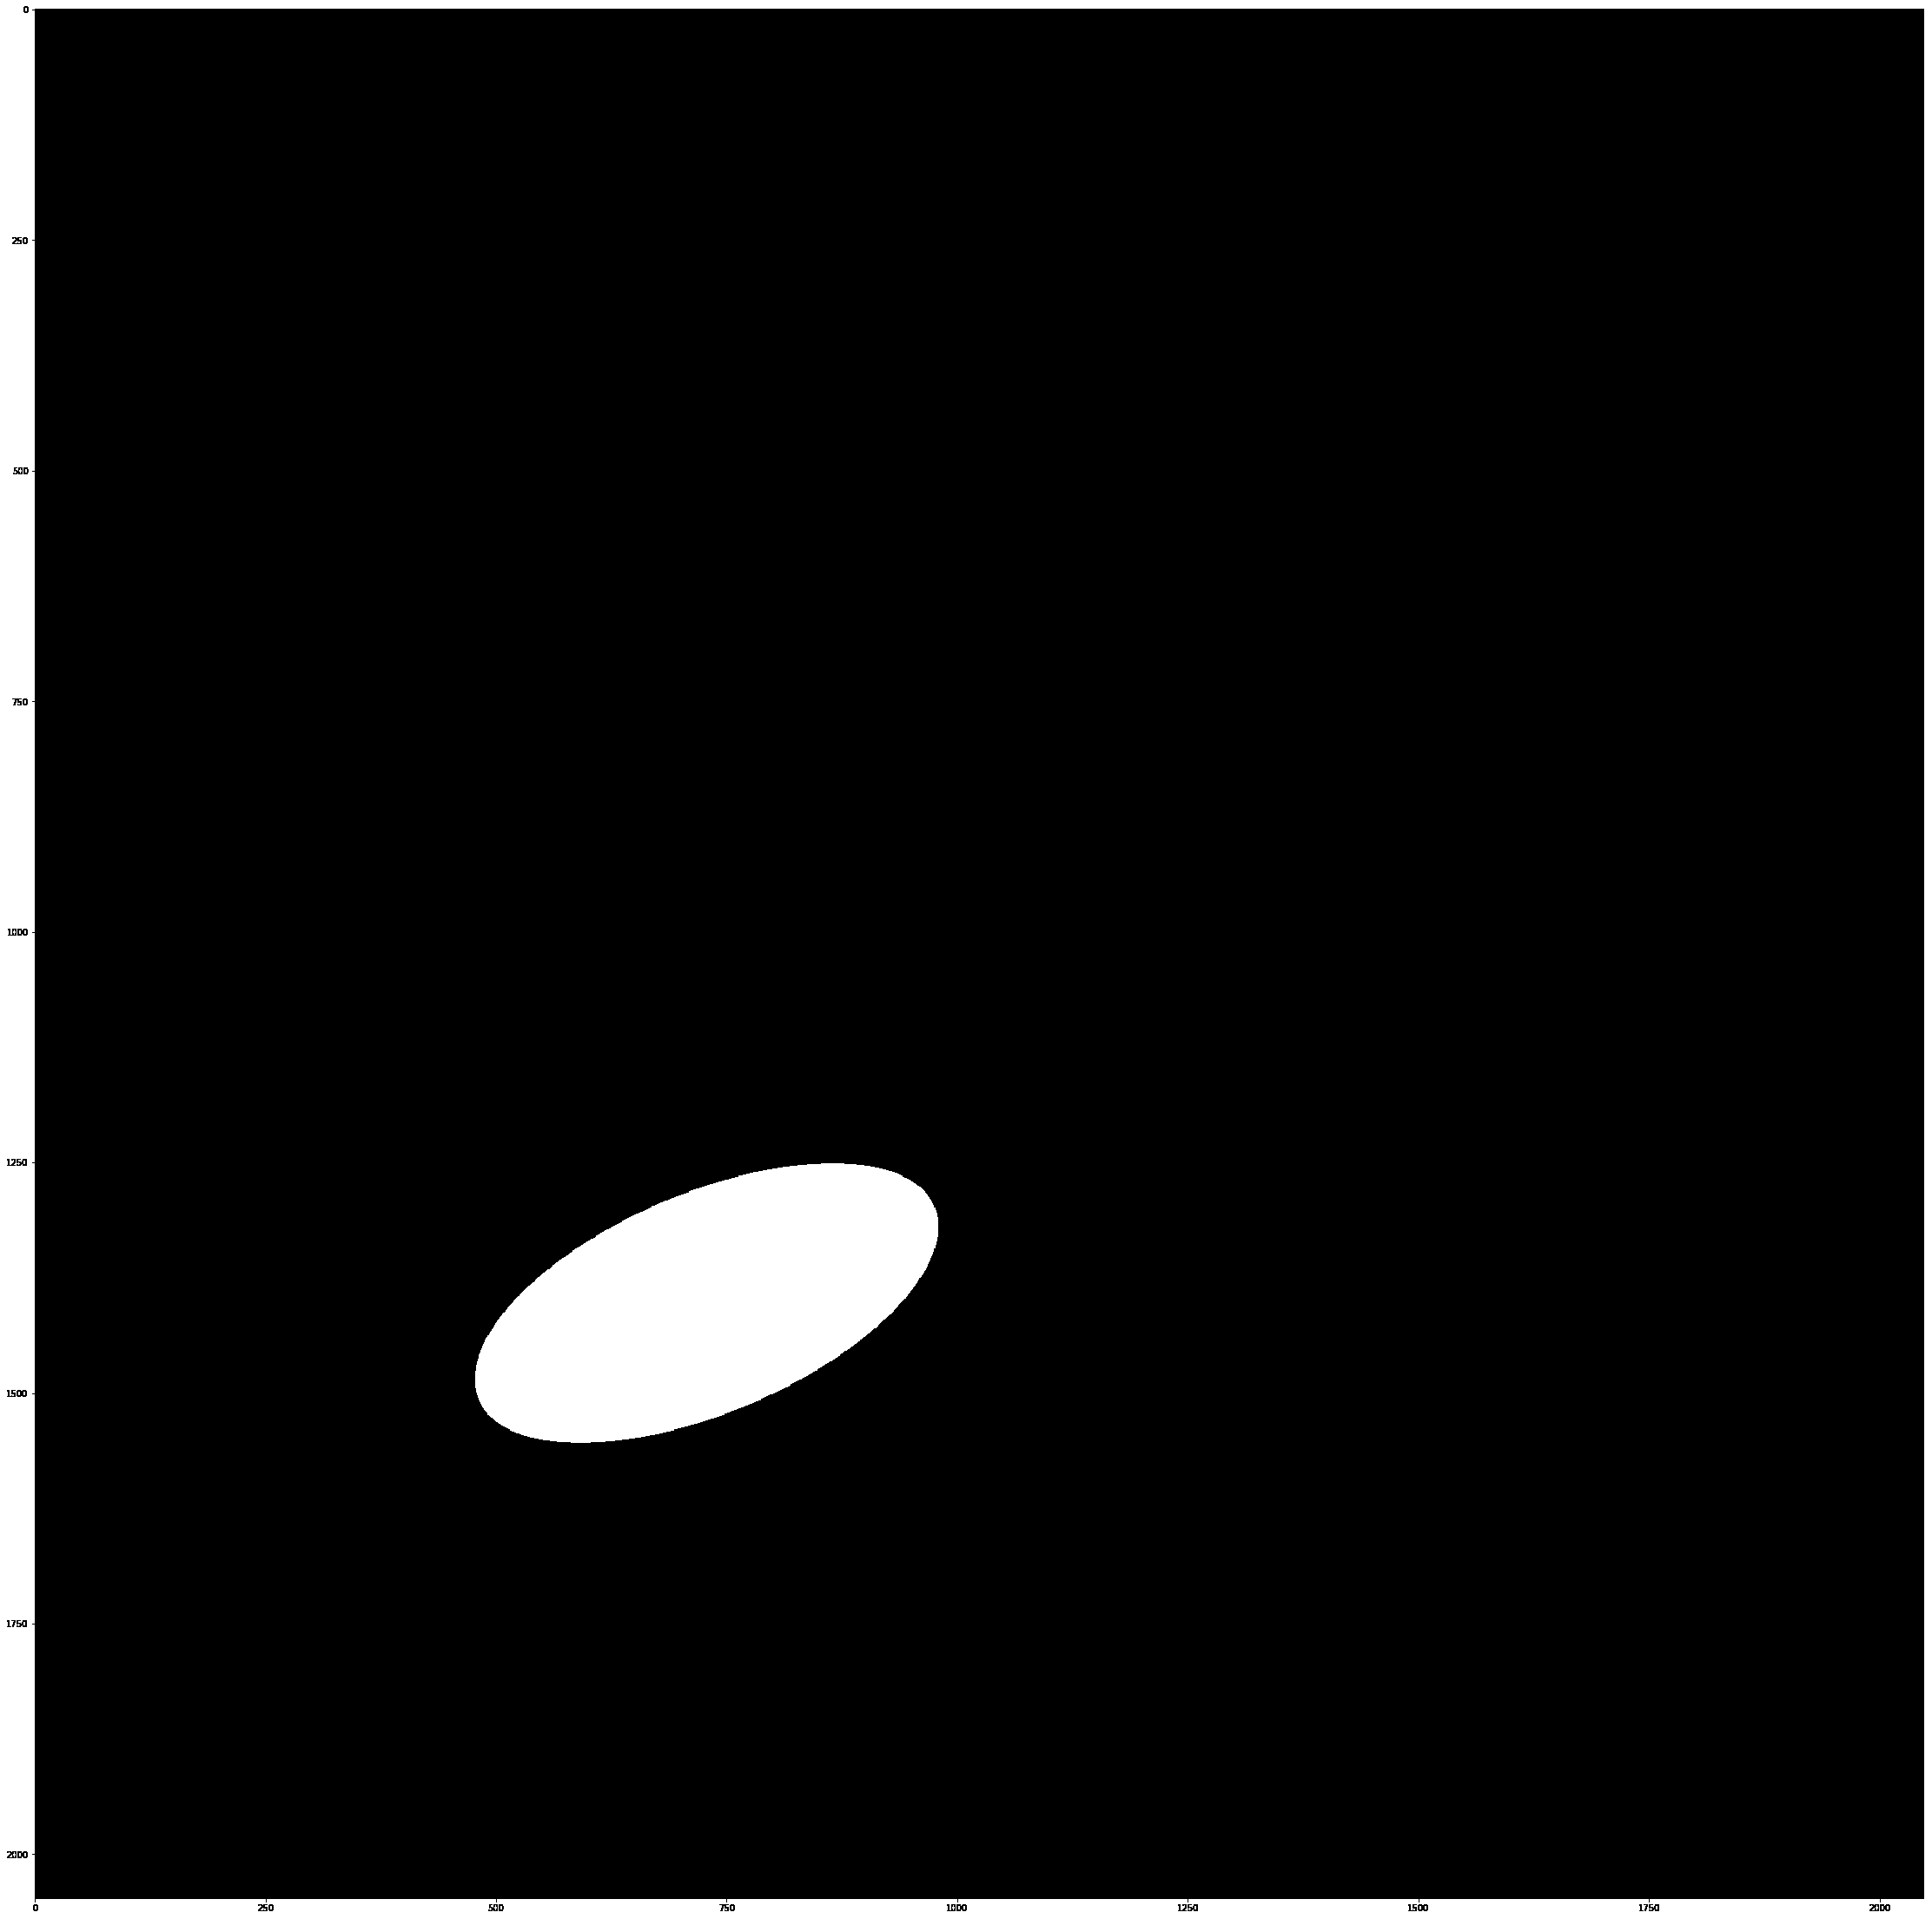
\includegraphics[width=0.6\linewidth]{mask0}}
    \caption{Пример маски для сегментации скопления. В разбиении с $n_{side} = 2^{17}$ были выбраны
        те пиксели, расстояние которых от центра скопления меньше $5'$}
\end{figure}

\section{Тангенциальная проекция}
Ещё один способ перенести данные со сферы на плоскость --- тангенциальная проекция WCS (World 
Coordinate Systems). Такая проекция сохраняет форму объектов, но искажает их площадь. Кроме того, 
такая проекция меняется в зависимости от выбранного центра проектирования объектов, и один и тот же
объект может попасть на разные проекции, что не всегда можно отследить. \\

Проекция HEALPix считается более удобной, так как она является абсолютной для всей области неба и 
для неё нет необходимости выбирать центр проекции.\\
